%-------------------------------------------------------------------------
%-------------------------------------------------------------------------
%-------------------------------------------------------------------------
\section{Evaluation}\label{sec:evaluation}
%-------------------------------------------------------------------------
\iffalse
\TODO{A key weakness is the lack of qualitative and quantitative comparisons with baselines. The only baseline algorithm compared against is the a modification of the full algorithm presented in the paper. There are many algorithms for segmentation of RGB images, RGBD images and meshes which could have been compared against. Consider some of the mesh segmentation algorithms presented in Chen et al, A Benchmark for 3D Mesh Segmentation, SIGGRAPH 2009. At least one of these algorithms could be used on your generated meshes with little modification. Consider also 'Mesh Segmentation with Concavity­Aware Fields' (Au et al., TVCG 2012).} \cite{Chen:2009:ABF, AZCXT11}

\TODO{Segmentation is a subjective problem, as a scene could be segmented into regions comprising semantic objects, or parts of objects, or segments of similar sizes etc. These different possible segmentation requirements are not addressed at all in the paper. As the labeling of the dataset is provided by the authors, the desired type of segmentation should be discussed in some way. For example, on the ground truth, it appears also that two of the branches of the tree are segmented as one object, but the others are segmented separately. It is not clear that there is an obvious 'ground truth' for the sequences presented without a discussion of the desired aim of the segmentation. Potential improvements discussed on line 538 could also be valuable.
}

\TODO{The authors state that they are not aware of benchmarks for scene segmentation from monocular video (line 532). The SUN3D dataset (http://sun3d.cs.princeton.edu/), while not directly designed for the problem in hand, comprises of an RGBD video with camera pose information and accompanying segmentations. Qualitative and quantitative results on a dataset such as this would help to convince reviewers of the strengths of the presented algorithm.} \cite{xiao2013sun3d}

\TODO{The experimental evaluation is incomplete. There is absolutely no quantitative nor qualitative comparison to state of the art methods on the 3d segmentation task. For fair comparison, the authors should use a standard dataset, such as:
­ the NYU dataset, from N. Silberman, D. Hoiem, P. Kohli, and R. Fergus. Indoor segmentation and support inference from rgbd images. In ECCV 2012. ­ the TUM dataset, from J. Sturm, N. Engelhard, F. Endres, W. Burgard, and D. Cremers. A benchmark for the evaluation of rgb­d slam systems. In IROS 2012.} \cite{Silberman:ECCV12, sturm12iros}

More dataset: Contextually Guided Semantic Labeling and Search for 3D Point Clouds, Abhishek Anand, Hema S. Koppula, Thorsten Joachims, Ashutosh Saxena. In IJRR, 2012

SCZ Scene parsing beyond Physics? Any recent relevant RSS papers?
\fi

\subsection{Comparison Methodology}\label{sec:comparison}
We are not aware of benchmarks for evaluating scene segmentation inferred
from monocular vision. While several RGB-D datasets for reconstruction and 
segmentation exist (such as \cite{xiao2013sun3d, Silberman:ECCV12, sturm12iros, anand2012contextually}) they
tend to have highly variable viewpoint scale, which makes the appropriate scale of a segmentation (based on occlusion cues) vary over time, in addition to having very similar scene content and geometry (indoor office and home scenes).
Therefore, we have captured a set of diverse sequences, both indoor and outdoor, 
on which to test our dense reconstruction and
segmentation pipeline, and included one provided by \cite{Graber2011}.
To generate ground truth for each sequence we manually segment the reconstruction into regions 
that correspond to objects at a scale appropriate for interaction from the video's perspective. As noted in section \ref{sec:sceneModel}, objects compose a nested
covering of sets, and the choice of which partition to use for groundtruth is subjective, though we have endeavored to select a fair partition into the
dominant objects as visible from the videos.
We compare the results of our occlusion-constrained segmentation to a baseline of segmentation using standard geometric homogeneity cues (described in section
\ref{sec:curvGeod}), for which typically a fixed scale parameter must be selected to perform
segmentation, chosen to preserve as many of the dominant objects as possible without over-segmenting them. 
Note that it is infeasible for a single scale to accurately segment the entire scene, necessitating 
our adaptation of scale using occlusion cues from the viewer's motion.
Baseline segmentations are compared numerically to object-level segmentations through F-score
and precision-recall metrics. F-scores are computed following standard methodology \cite{OB14b},
to determine the agreement between ground-truth segments and computed segments.

Given a correspondence between computed cluster $c_i,\,i\in I$ and
ground-truth regions $g_j,\,j\in J$, we compute F-scores as follows.
Precision $P_{ij}$ and recall $R_{ij}$ are computed as the average (weighted by cluster size)
ground-truth fraction of clusters,
$P_{ij}=|c_i \cap g_j|/|c_i|$, which penalizes under-segmentation,
and the fraction of the corresponding ground-truth region covered by a cluster,
$R_{ij}=|c_i \cap g_j|/|g_j|$, which penalizes over-segmentation.
A compromise measure $F_{ij} = {2P_{ij}R_{ij}}/({P_{ij}+R_{ij}})$ penalizes both.
An optimal correspondence $\phi:I\to J$ is found by the Hungarian algorithm,
maximizing the the total F-score, 
\begin{equation}
F = \max_{\{\phi:I\to J\}}\tfrac{1}{|I|}\sum\nolimits_{i\in I} F_{i\phi(i)}.
\end{equation}

A precision-recall curve may also be computed by comparing a thresholded affinity
matrix $\delta_{M_{ij}>t}$ with the ground truth affinity matrix $\delta_{g_i=g_j}$. Since this is a 
monotonic function of distance along the scene, the precision-recall curve sampling over 
affinity thresholds allows us to evaluate the segmentation results across a range of scales. 



%-------------------------------------------------------------------------
\subsection{Geometric and Occlusion-Constrained Segmentation Results}\label{sec:results}
We present results in the form of re-projected segmentations and sample geodesics on four geometrically and topologically complex scenes, three of which were
collected outdoors (Park, Industrial1, and Industrial2) and two of which contain notable multi-scale geometry (Park and City of Sights (CoS), made available by \cite{Graber2011}). Please refer to our supplemental material for video results on these sequences. 

Fig. \ref{fig:gtSegs} shows sample images and re-projected groundtruth segmentations for each scene, Fig. \ref{fig:detObjs} shows sample occlusion-based image segmentation results, and Fig. \ref{fig:adaptTravs} shows sample occlusion-constrained geodesics on the scene built using the occlusion-based image segmentations. Fig. \ref{fig:geoSegs} shows qualitative examples of our baseline geometric segmentation. Fig. \ref{fig:ourSegs} shows qualitative examples of our final scene segmentations, with numerical evaluations relative to groundtruth shown in Fig. \ref{fig:numericalEval}.

In the CoS sequence the multi-scale geometry of the domed structure (a single object) makes the selection of a single scale infeasible, 
however the adaptive geodesic is able to shape distances on the scene based on the available image segmentations, enabling a correct segmentation. The Park sequence shows a scene with complex natural geometry on the ground and smoothly varying geometry on the nearby
tree. Highly variable ground geometry makes the selection of a single scale unable to correctly segment both the smooth tree
limbs (which occlude each other throughout the sequence) and the rough ground (as a single object).
These sequences demonstrate that adapting the geometry using
occlusion-based image segmentation enables segmentation at the appropriate viewpoint scale for all dominant objects in the scene. Both
Industrial sequences shows scenes of sophisticated
topology and geometry, the segmentation of which is improved using our occlusion-informed geometry compared to the over-segmented results using 
standard geometric approaches.


The quantitative evaluation of Fig. \ref{fig:numericalEval} demonstrates a consistent improvement
over a standard geometric segmentation when compared to our adaptive geodesic.
The Precision-Recall curve comparisons serve to provide further support to the claim that no fixed scale treatment of purely geometric distances can correctly segment scenes with complex geometry, as varying affinity scale
for both methods typically shows an increase in performance for our adaptive geodesic distances.

Fig. \ref{fig:timing} shows a summary of timings for the various components of our system. Typical
size of meshes used to represent the scene geometry are on the order of fifty thousand, with
coarsified meshes for image segmentation on the order of two thousand, and subgraphs used for
clustering on the order of several hundred. The entire system runs on a 3.5Ghz desktop
machine (dense reconstruction, image, and scene segmentation).

\begin{figure}
\begin{center}
 \centerline
      {
        \hbox
            {%\\
              \begin{tabular}{cc}
		        {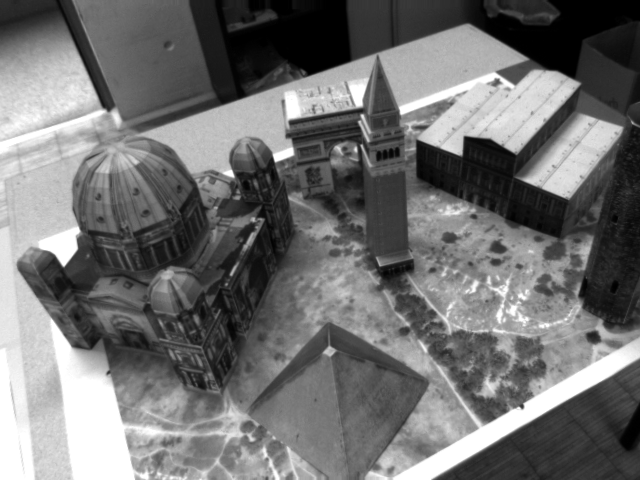
\includegraphics[width=0.4\textwidth]{figs/cos/im_0001.png}}
        		{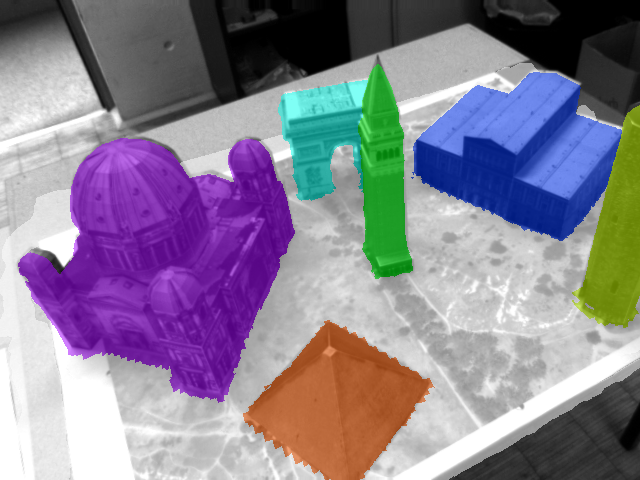
\includegraphics[width=0.4\textwidth]{figs/cos/gtseg_0001.png}}
        		\\
        		{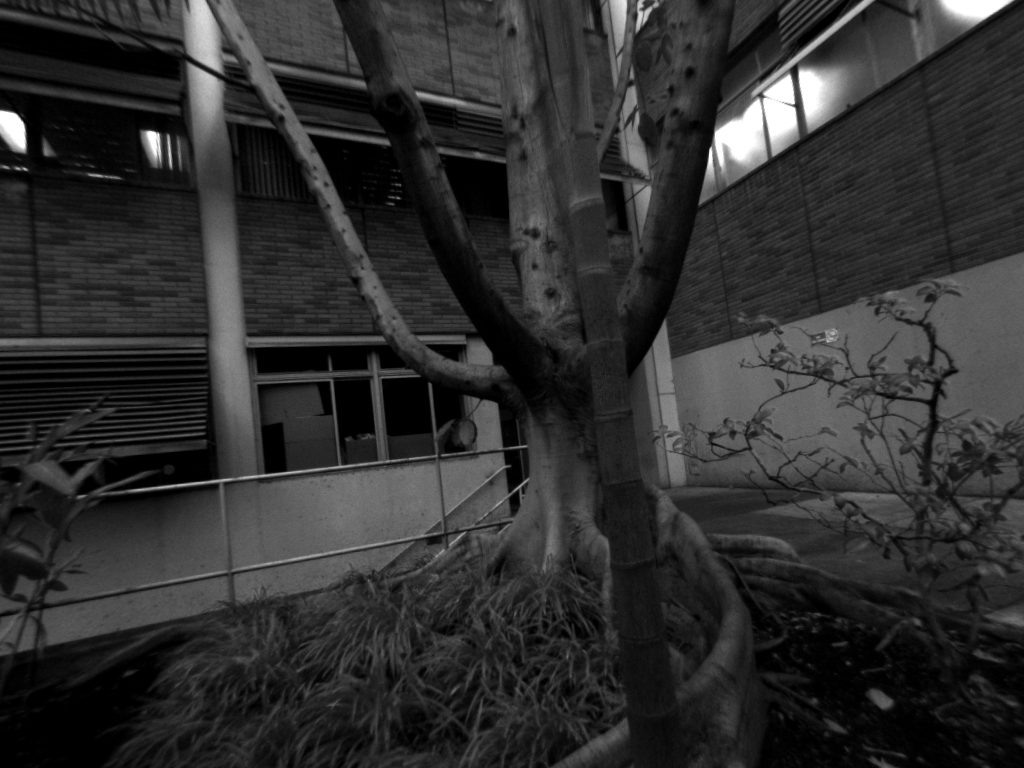
\includegraphics[width=0.4\textwidth]{figs/park4/im_0024.png}}
        		{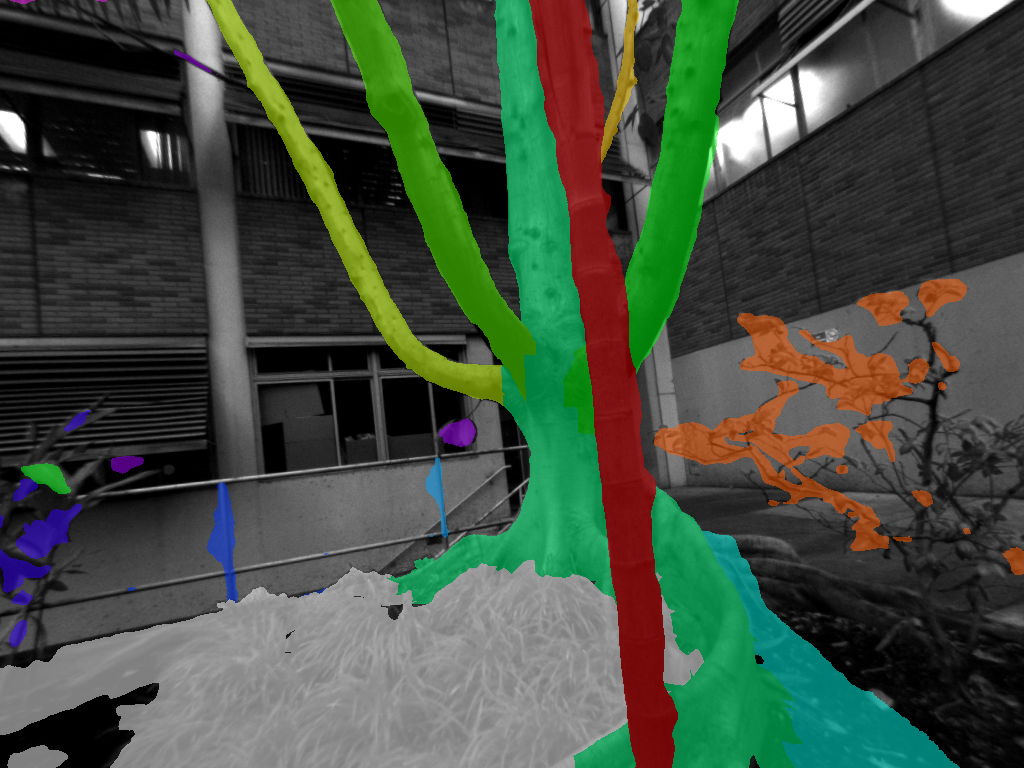
\includegraphics[width=0.4\textwidth]{figs/park4/gtseg_0024.png}}
        		\\
        		{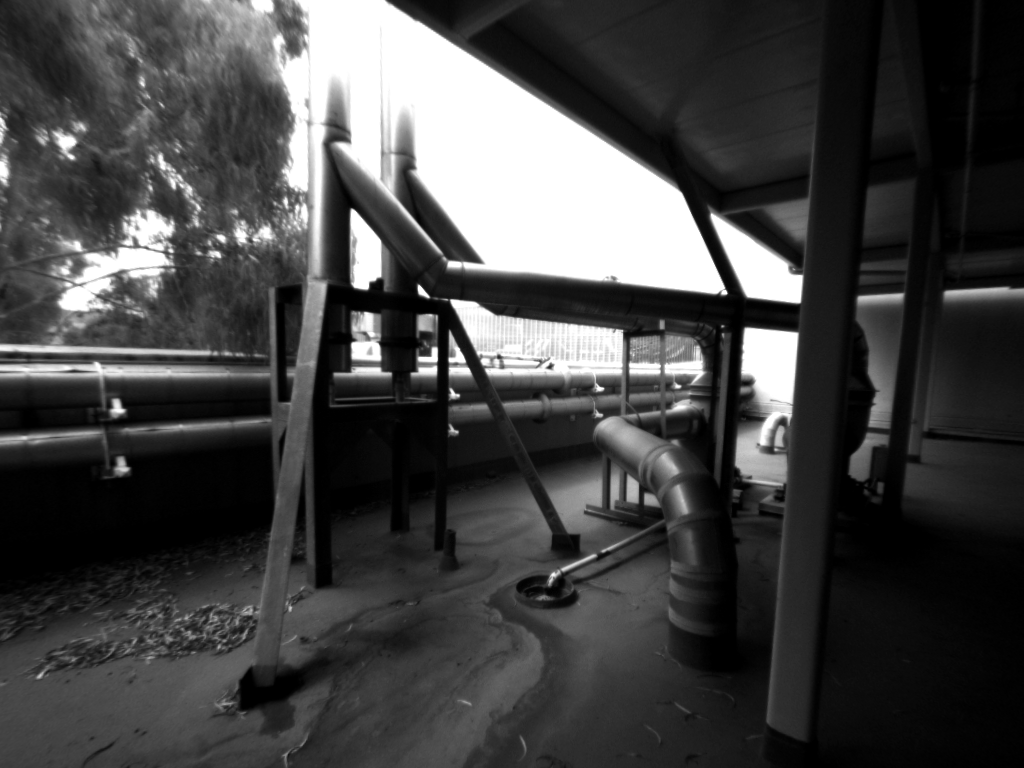
\includegraphics[width=0.4\textwidth]{figs/pipes2/im_0059.png}}
        		{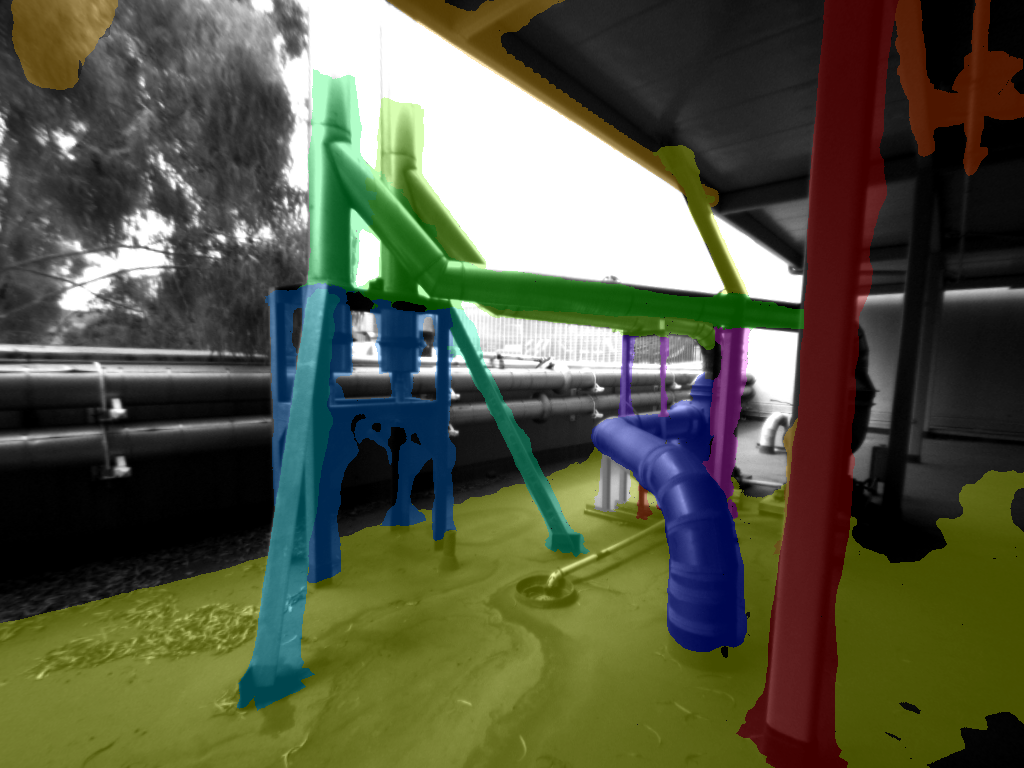
\includegraphics[width=0.4\textwidth]{figs/pipes2/gtseg_0059.png}}
        		\\
        		{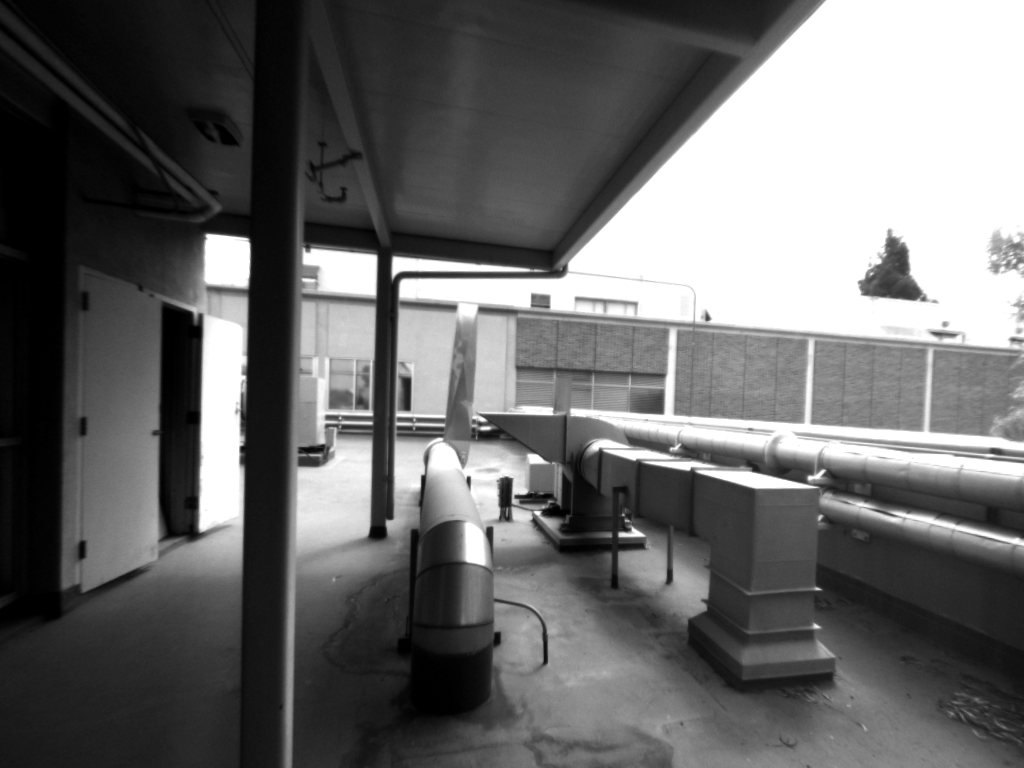
\includegraphics[width=0.4\textwidth]{figs/pipes3/im_0007.png}}
        		{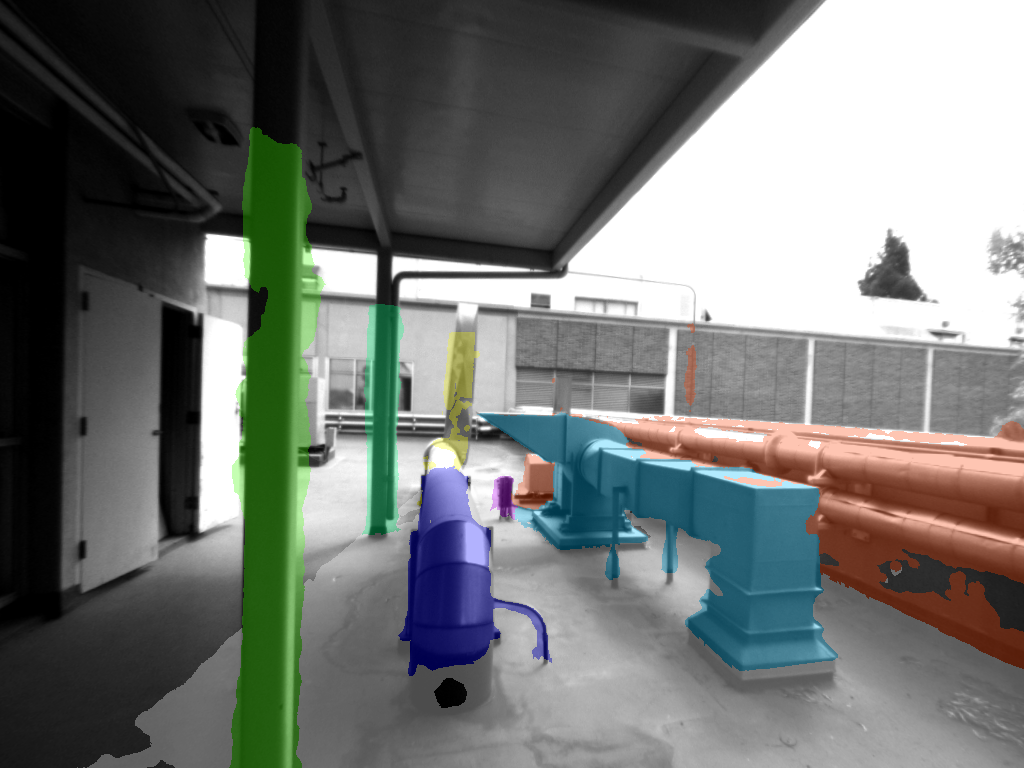
\includegraphics[width=0.4\textwidth]{figs/pipes3/gtseg_0007.png}}
              \end{tabular}
            }
      }
\end{center}
   \caption{\small Sample frames (left) and re-projected groundtruth segmentations (right) for CoS (top), Park, Industrial1, Industrial2 (bottom). Different colors indicate different segments.}
\label{fig:gtSegs}
\end{figure}

\begin{figure}
\begin{center}
 \centerline
      {
        \hbox
            {%\\
              \begin{tabular}{cc}
		        {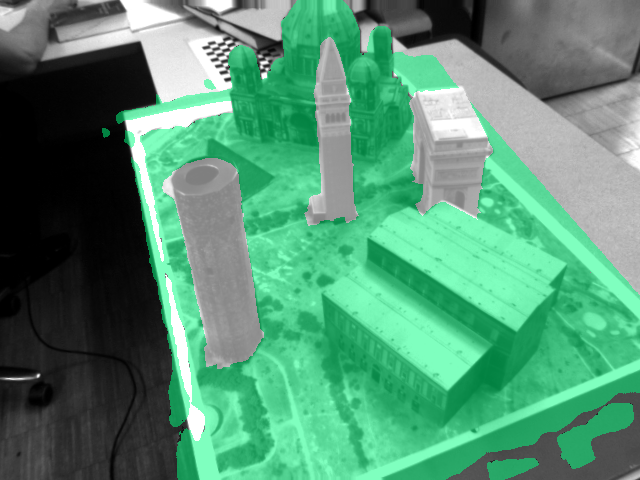
\includegraphics[width=0.4\textwidth]{figs/cos/det_0024.png}}
        		{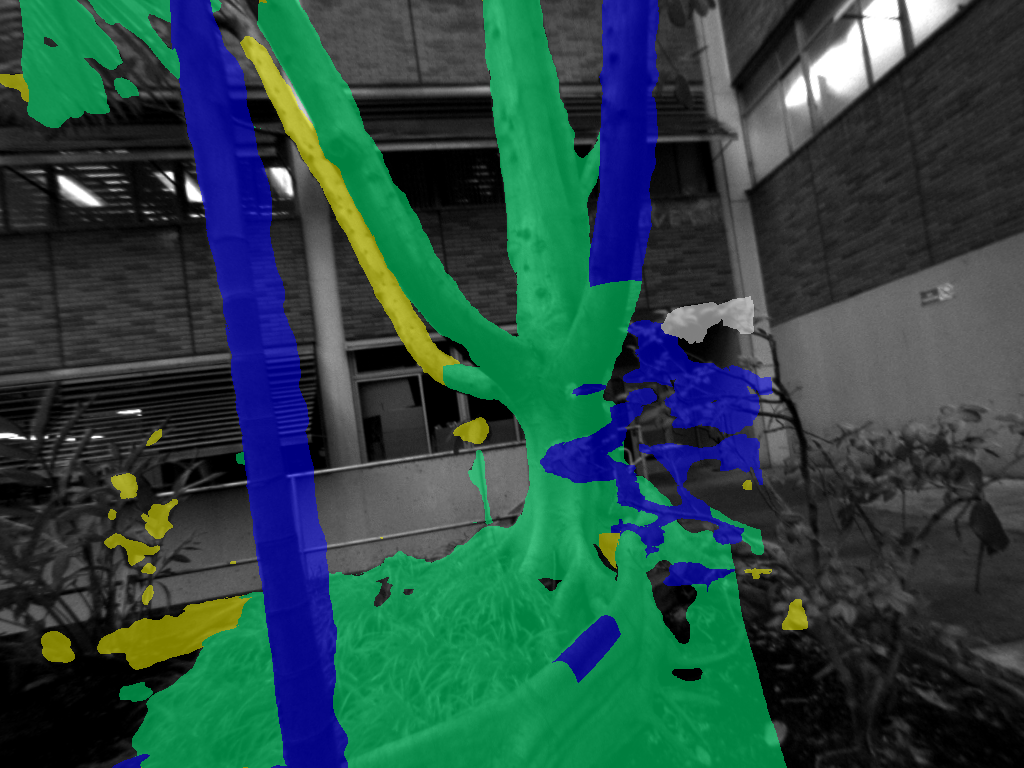
\includegraphics[width=0.4\textwidth]{figs/park4/det_0034.png}}
        		\\
        		{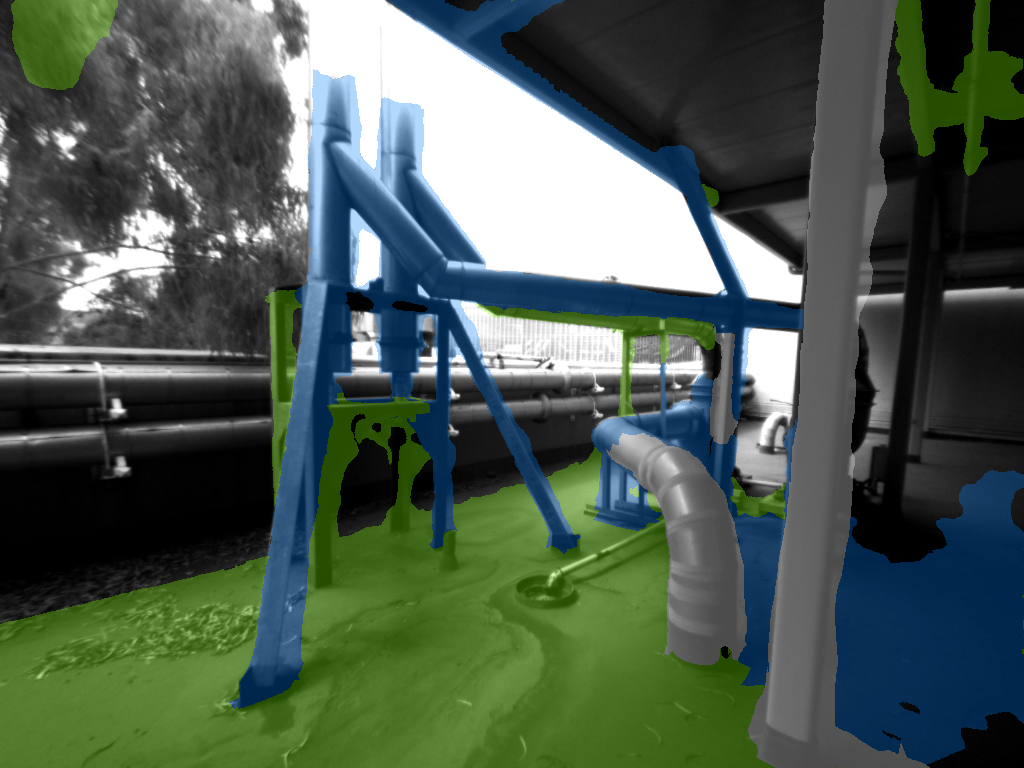
\includegraphics[width=0.4\textwidth]{figs/pipes2/det_0059.png}}
        		{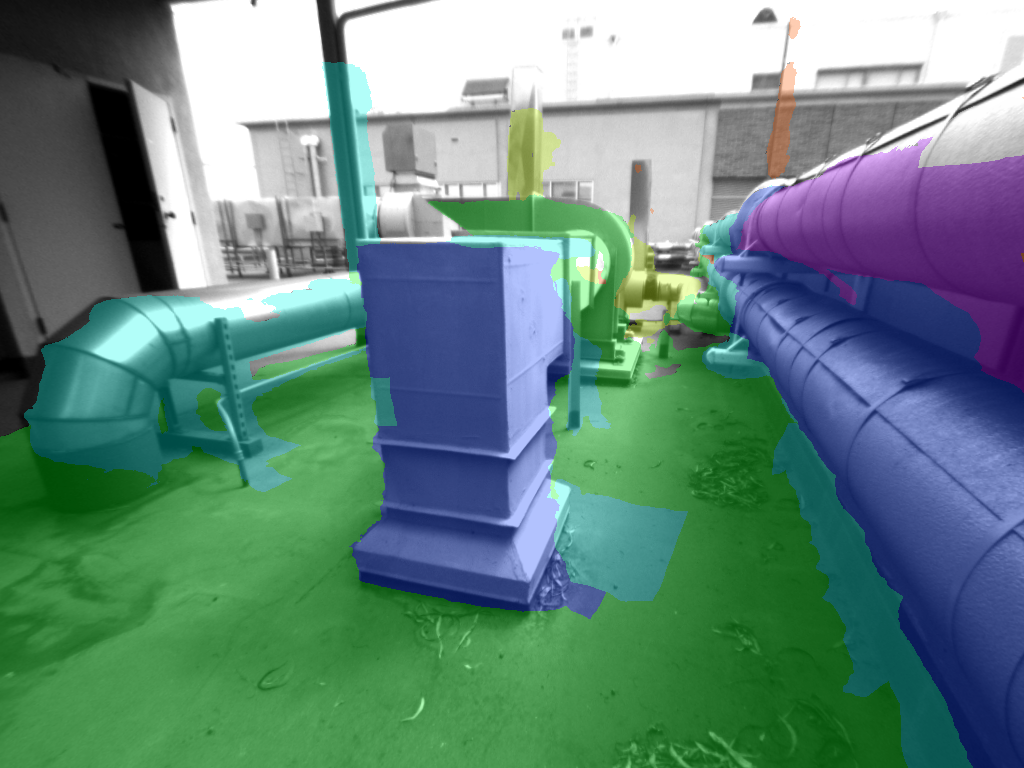
\includegraphics[width=0.4\textwidth]{figs/pipes3/det_0081.png}}
              \end{tabular}
            }
      }
\end{center}
   \caption{\small Sample single-image segmentation on frames from CoS (top left), Park (top right), Industrial1 (bottom left), Industrial2 (bottom right) inferred as described in Sec. \ref{sec:signatures}. Different colors indicate different segments from occlusion-guided segmentation.}
\label{fig:detObjs}
\vspace{-0.1in}
\end{figure}

\begin{figure}
\begin{center}
 \centerline
      {
        \hbox
            {%\\
              \begin{tabular}{cc}
		        {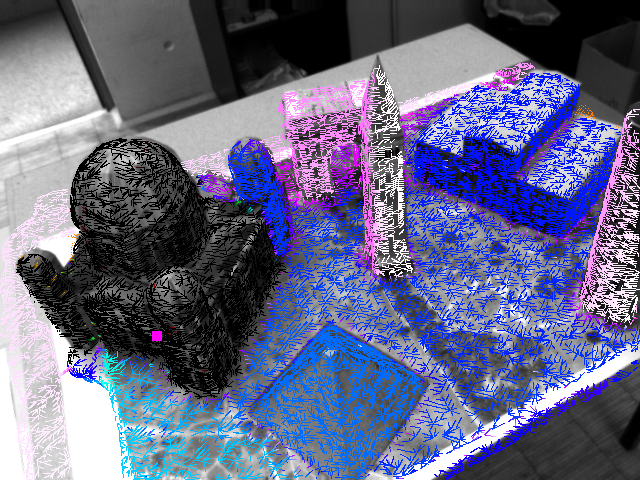
\includegraphics[width=0.4\textwidth]{figs/cos/tra_0024.png}}
        		{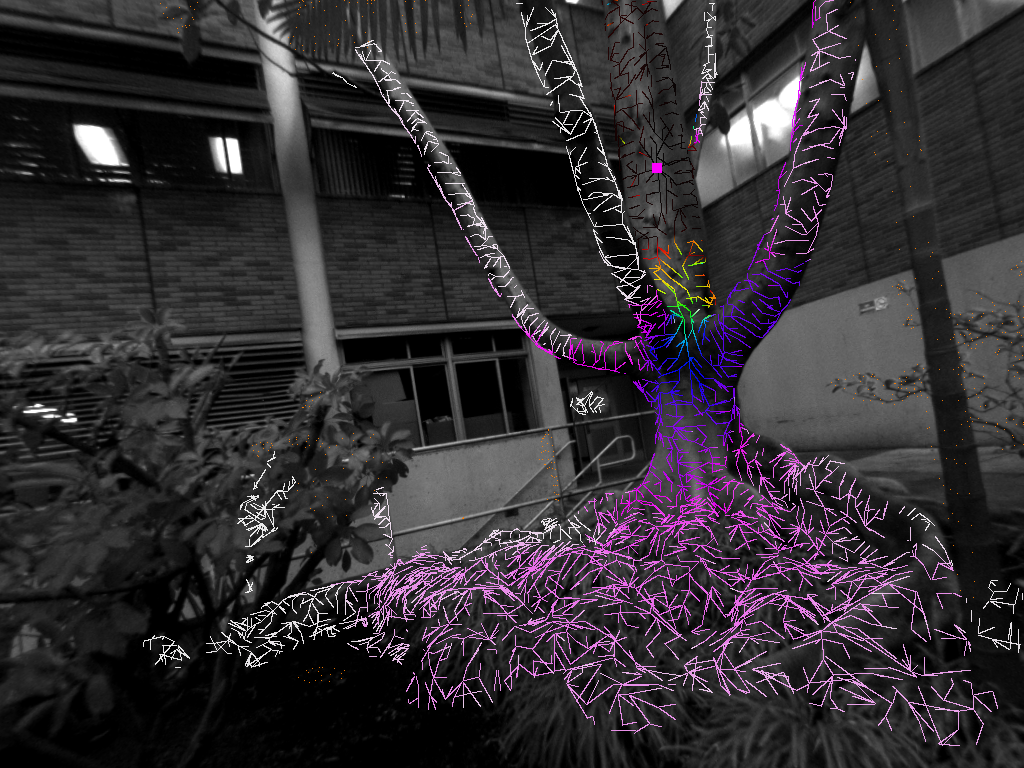
\includegraphics[width=0.4\textwidth]{figs/park4/tra_0072.png}}
        		\\
        		{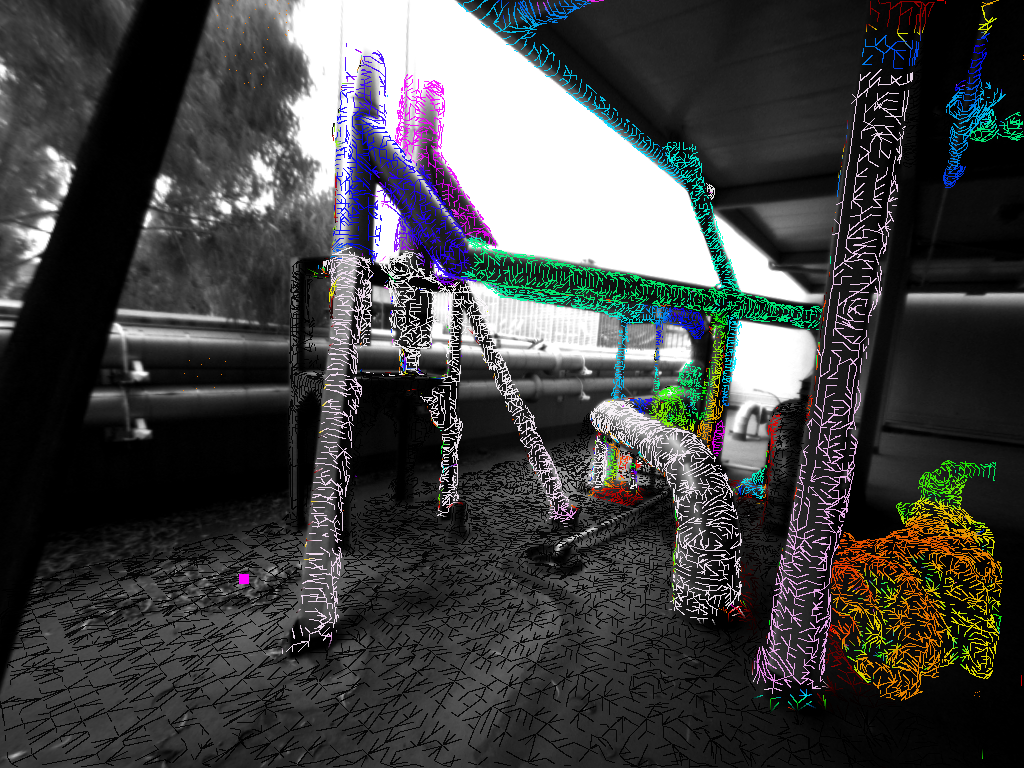
\includegraphics[width=0.4\textwidth]{figs/pipes2/tra_0003.png}}
        		{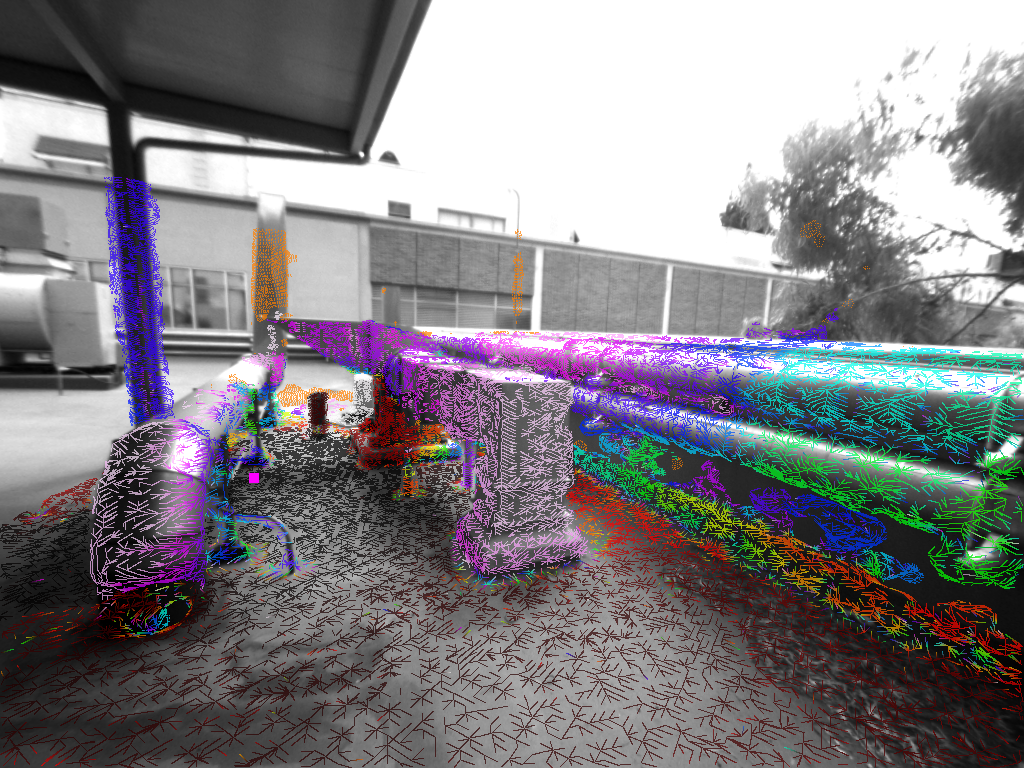
\includegraphics[width=0.4\textwidth]{figs/pipes3/tra_0059.png}}
              \end{tabular}
            }
      }
\end{center}
   \caption{\small Sample occlusion-constrained geodesics on CoS (top left), Park (top right), Industrial1 (bottom left), Industrial2 (bottom right) built as described in Sec. \ref{sec:adaptiveGeo}. Colored lines indicate the path of the geodesic on the scene originating at the magenta square in each image, with distance coded between zero (black) and one (white) through intervening colors.}
\label{fig:adaptTravs}
\end{figure}

\begin{figure}
\begin{center}
 \centerline
      {
        \hbox
            {%\\
              \begin{tabular}{cc}
		        {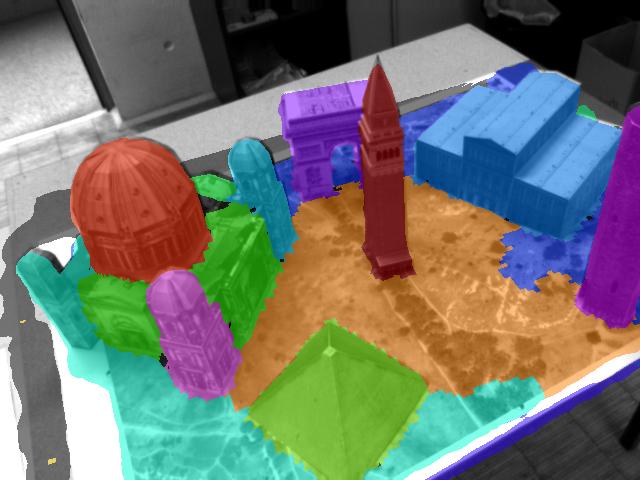
\includegraphics[width=0.4\textwidth]{figs/cos/geoseg_0001.png}}
        		{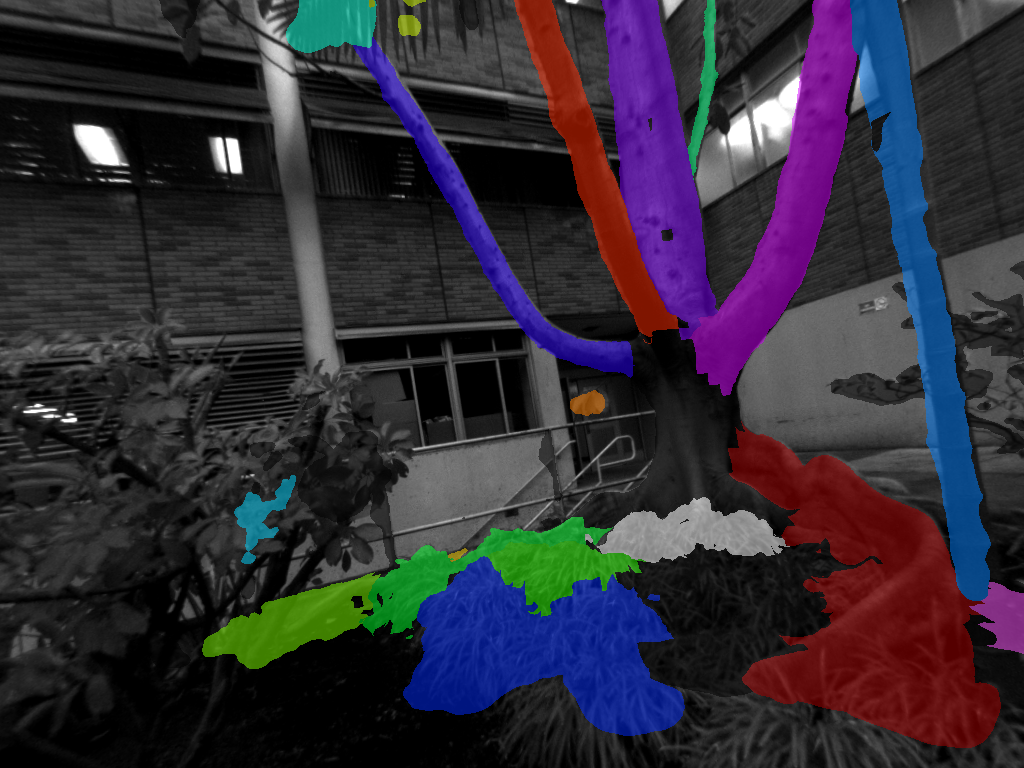
\includegraphics[width=0.4\textwidth]{figs/park4/geoseg_0001.png}}
        		\\
        		{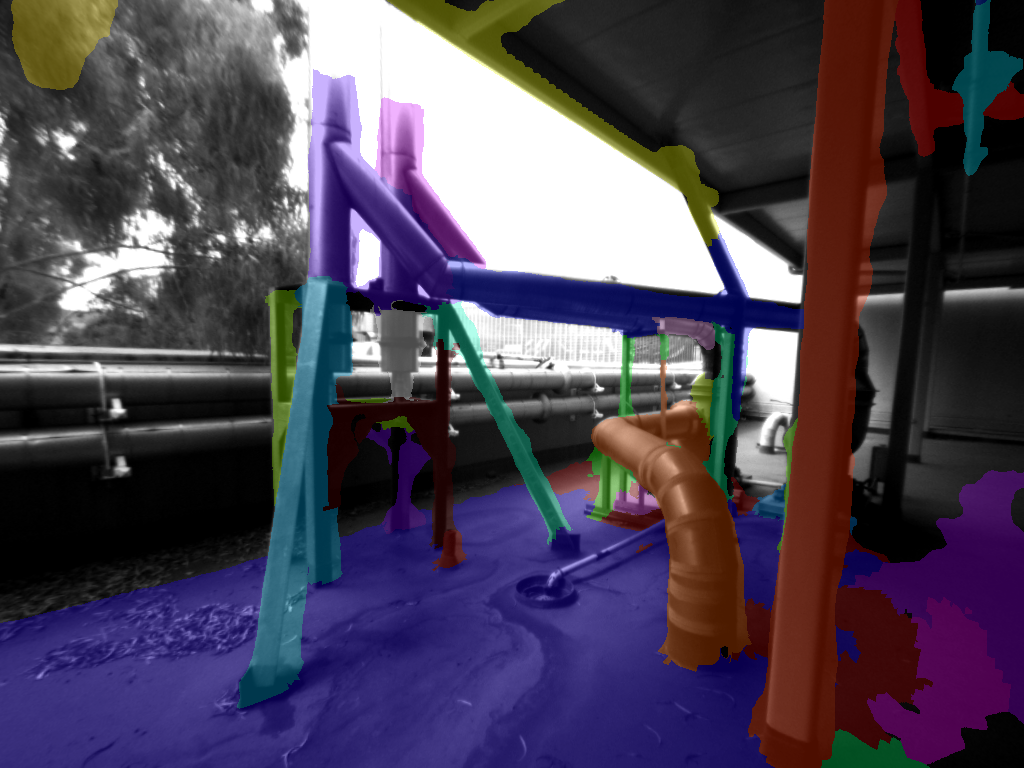
\includegraphics[width=0.4\textwidth]{figs/pipes2/geoseg_0059.png}}
        		{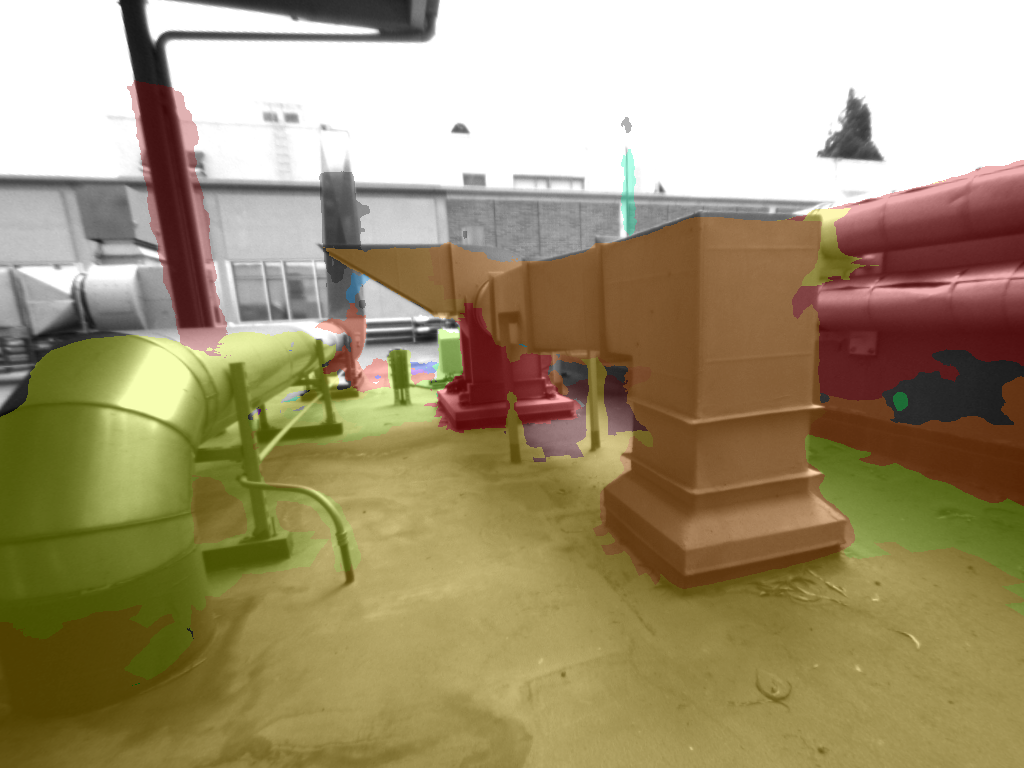
\includegraphics[width=0.4\textwidth]{figs/pipes3/geoseg_0065.png}}
              \end{tabular}
            }
      }
\end{center}
   \caption{\small Sample re-projections of our baseline geometric segmentation on CoS (top left), Park (top right), Industrial1 (bottom left), Industrial2 (bottom right). Different colors indicate different segments.}
\label{fig:geoSegs}
\end{figure}

\begin{figure}
\begin{center}
 \centerline
      {
        \hbox
            {%\\
              \begin{tabular}{cc}
		        {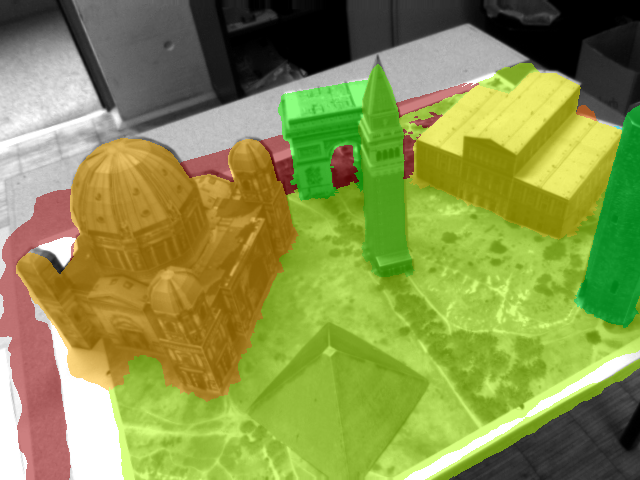
\includegraphics[width=0.4\textwidth]{figs/cos/sceneseg_0001.png}}
        		{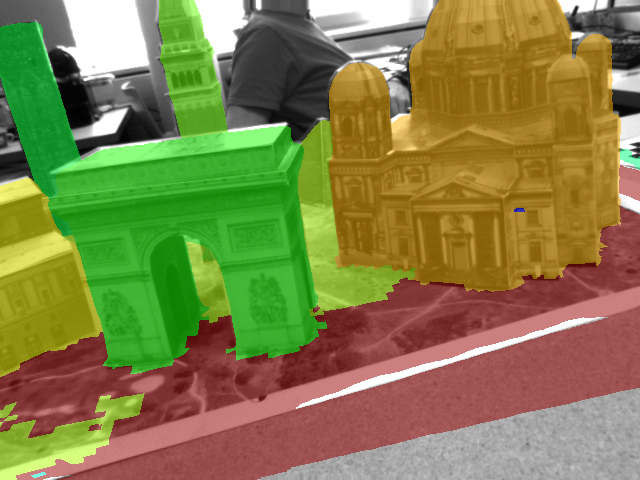
\includegraphics[width=0.4\textwidth]{figs/cos/sceneseg_0150.png}}
        		\\
        		{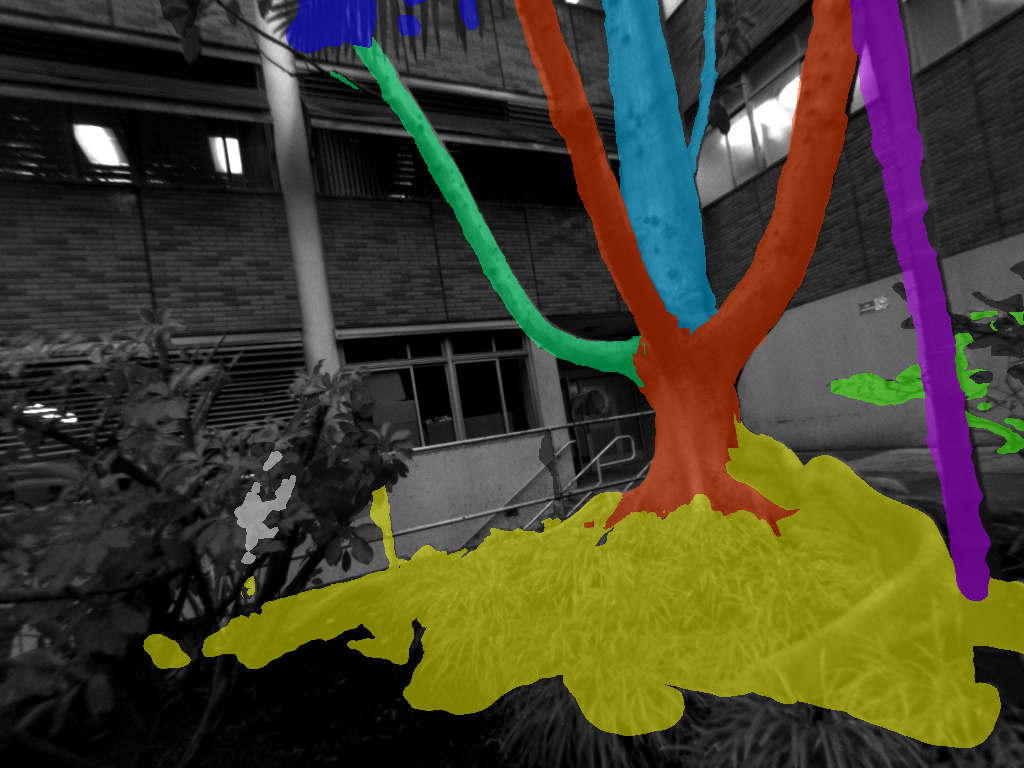
\includegraphics[width=0.4\textwidth]{figs/park4/sceneseg_0001.png}}
        		{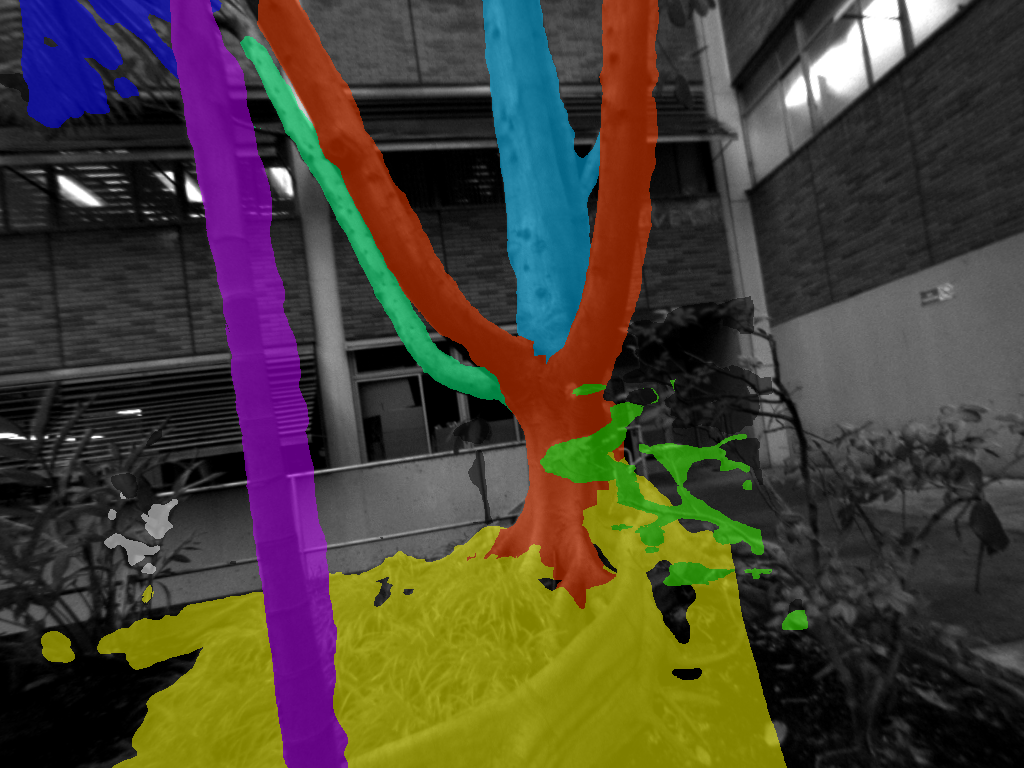
\includegraphics[width=0.4\textwidth]{figs/park4/sceneseg_0034.png}}
        		\\
        		{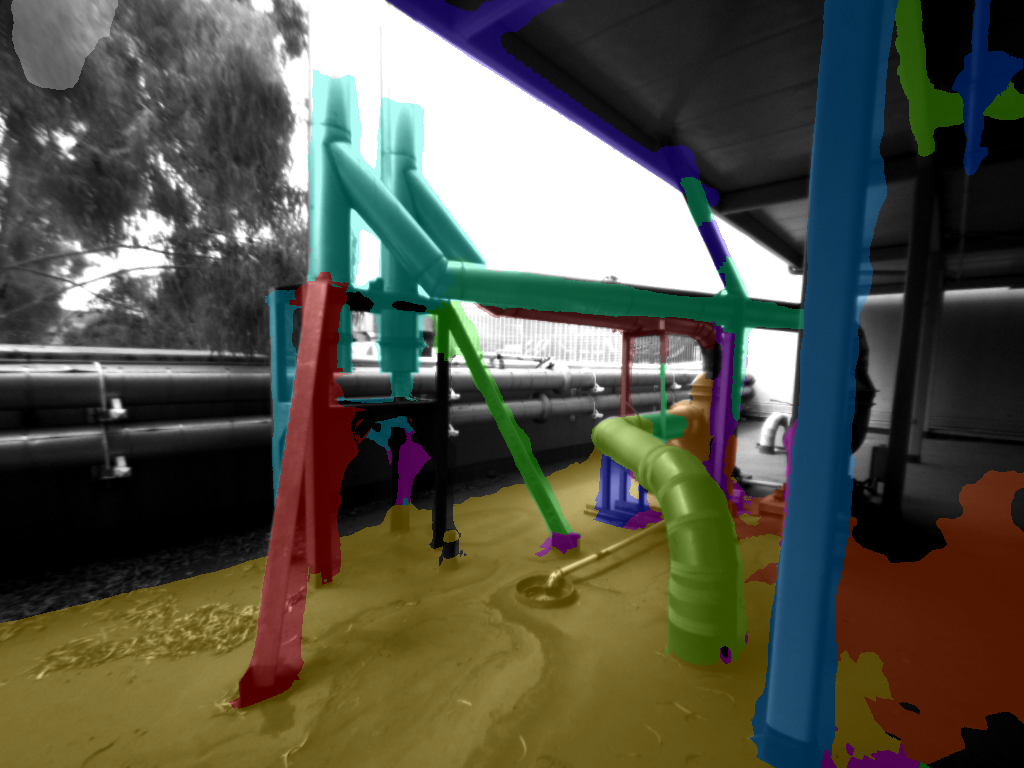
\includegraphics[width=0.4\textwidth]{figs/pipes2/sceneseg_0059.png}}
        		{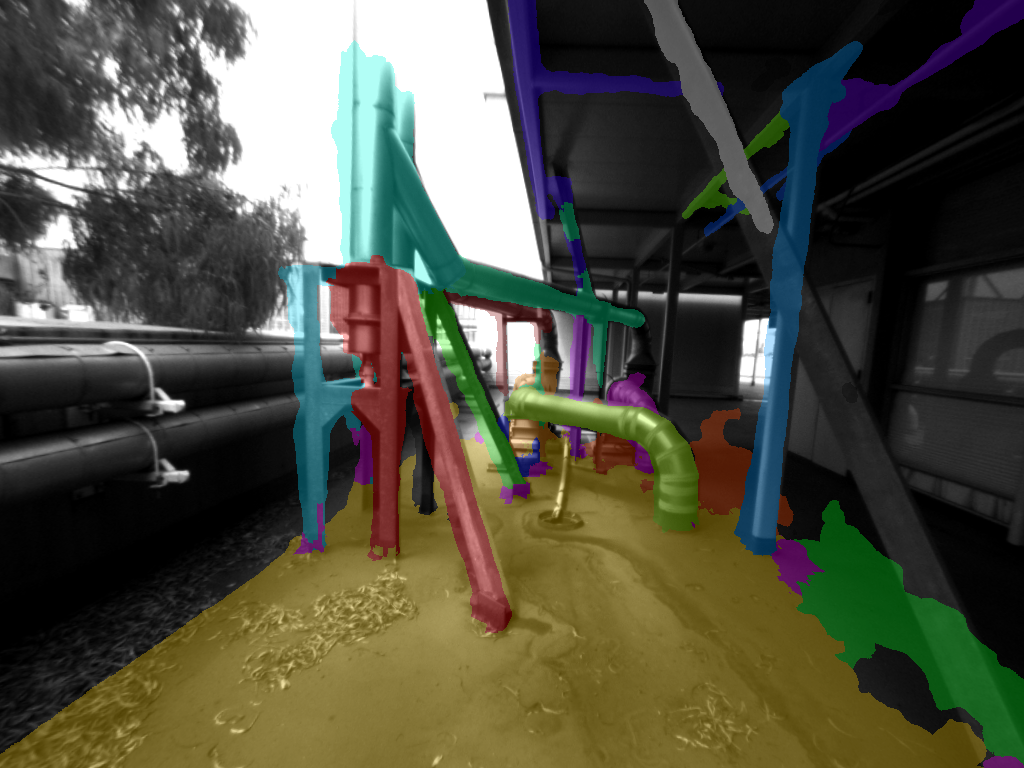
\includegraphics[width=0.4\textwidth]{figs/pipes2/sceneseg_0045.png}}
        		\\
        		{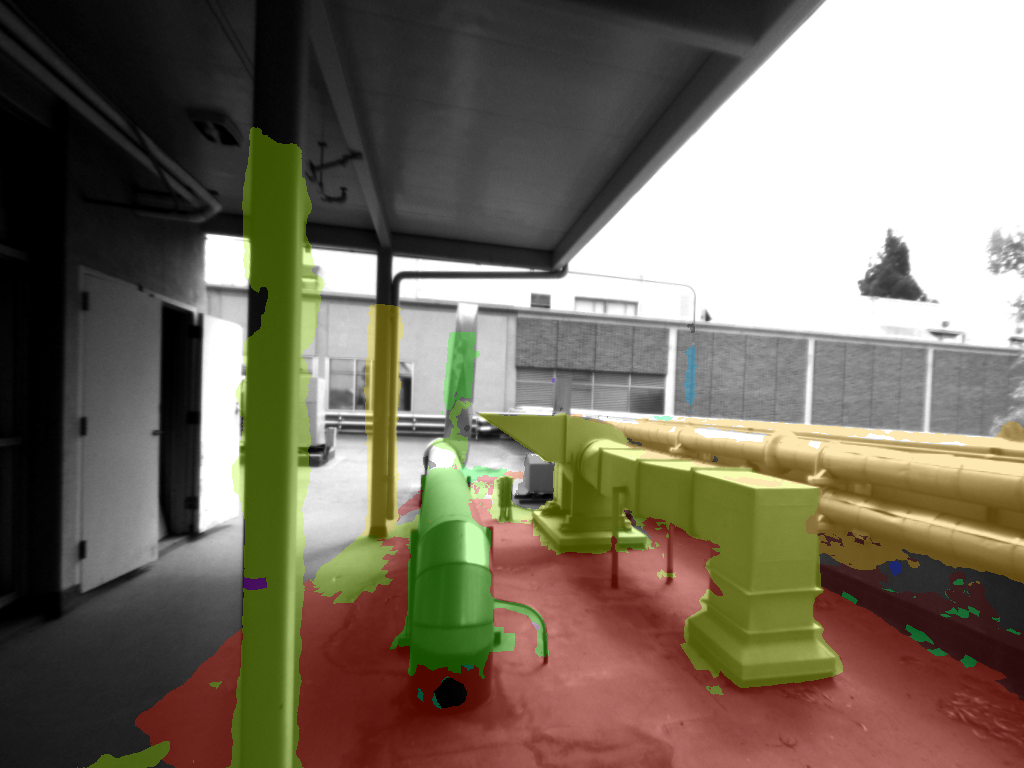
\includegraphics[width=0.4\textwidth]{figs/pipes3/sceneseg_0007.png}}
        		{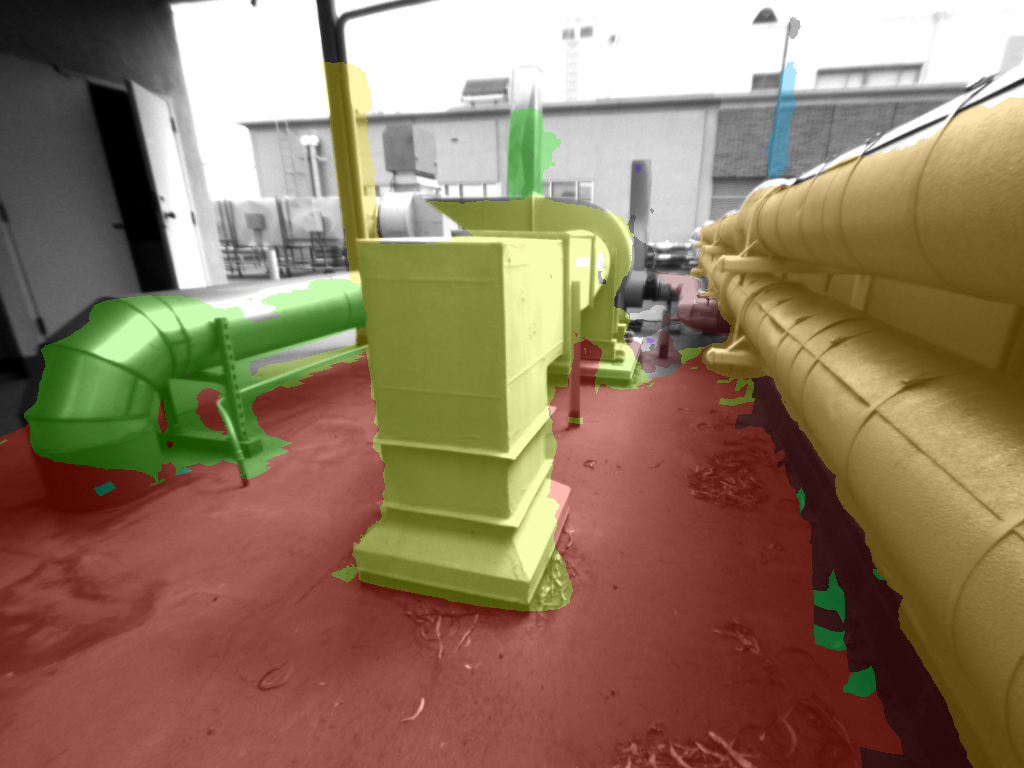
\includegraphics[width=0.4\textwidth]{figs/pipes3/sceneseg_0081.png}}
              \end{tabular}
            }
      }
\end{center}
{}
   \caption{\small Sample re-projected segmentation results using our occlusion-constrained geodesics for CoS (top), Park, Industrial1, Industrial2 (bottom). Different colors indicate different segments.}
\label{fig:ourSegs}
{}
\end{figure}
\begin{figure}
\begin{center}
\centerline
      {
        \hbox
            {%\\
              \begin{tabular}{cc}
	      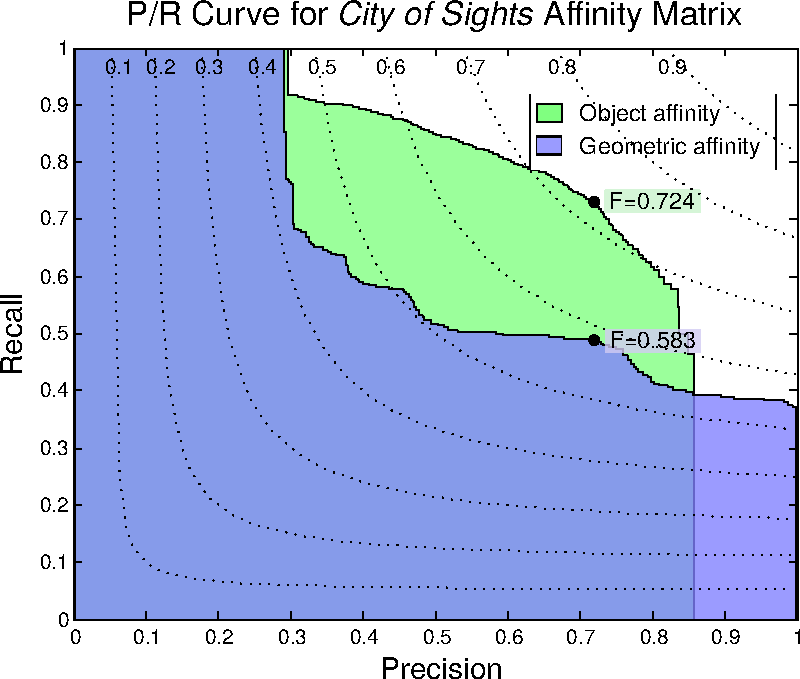
\includegraphics[width=0.4\textwidth]{figs/cos/validation.pdf}
	      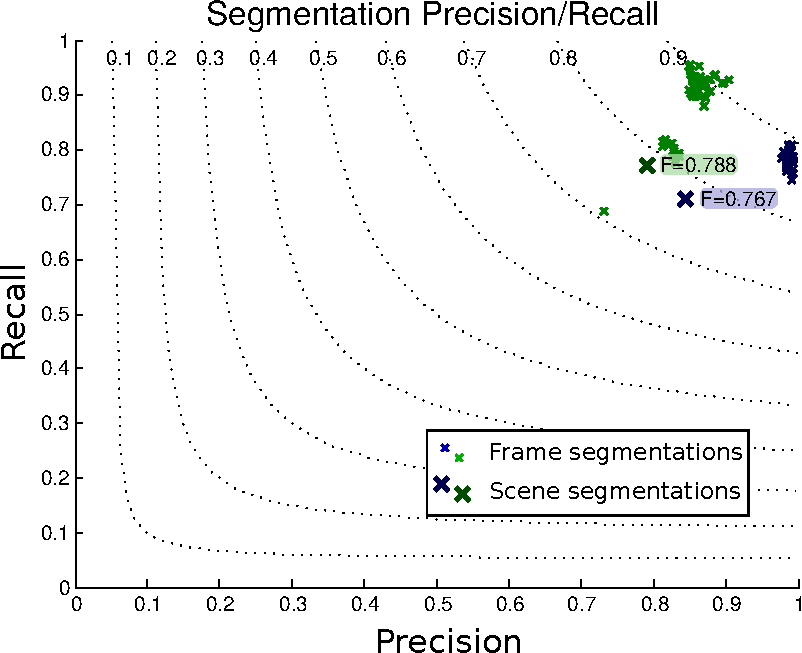
\includegraphics[width=0.4\textwidth]{figs/cos/frame_validation.pdf}
	      \\
	      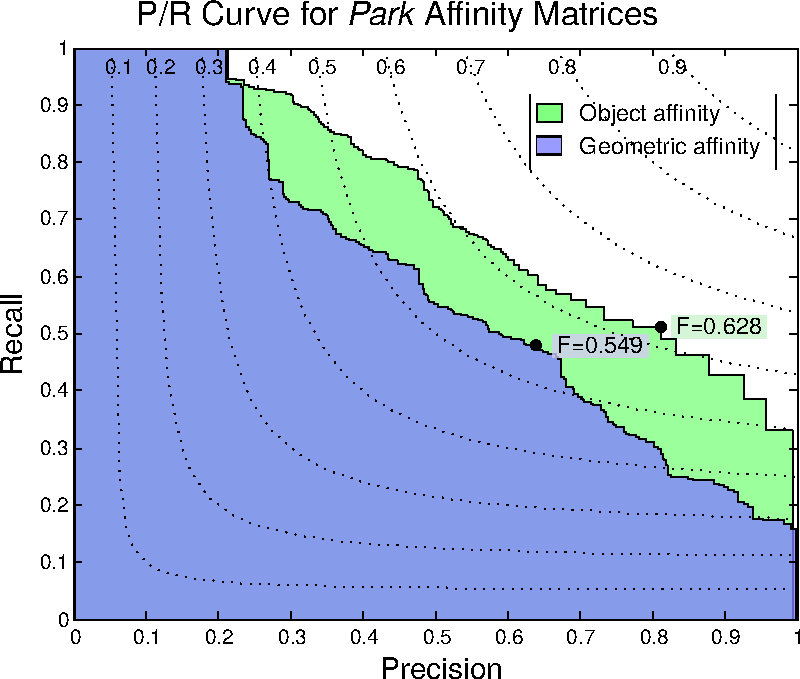
\includegraphics[width=0.4\textwidth]{figs/park4/validation.pdf}
	      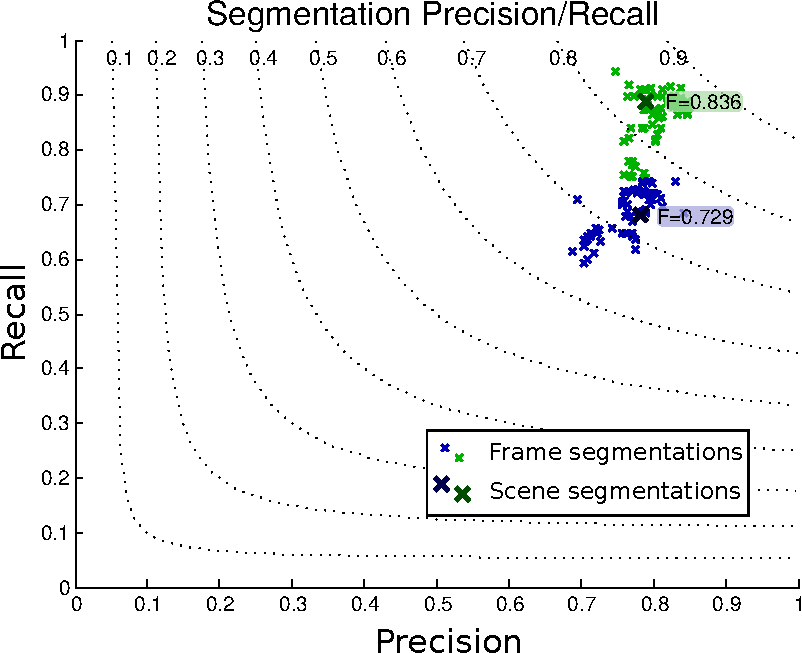
\includegraphics[width=0.4\textwidth]{figs/park4/frame_validation.pdf}
	      \\
	      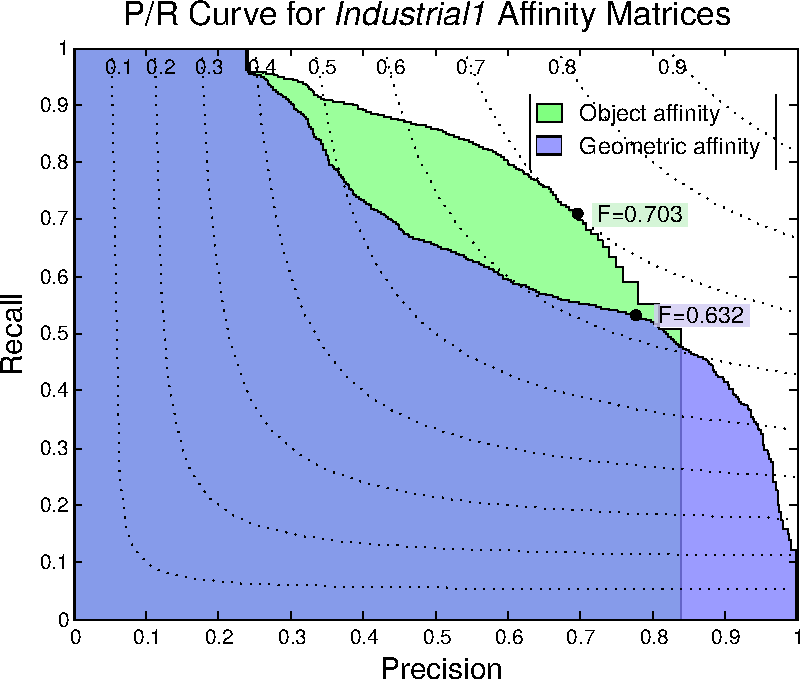
\includegraphics[width=0.4\textwidth]{figs/pipes2/validation.pdf}
	      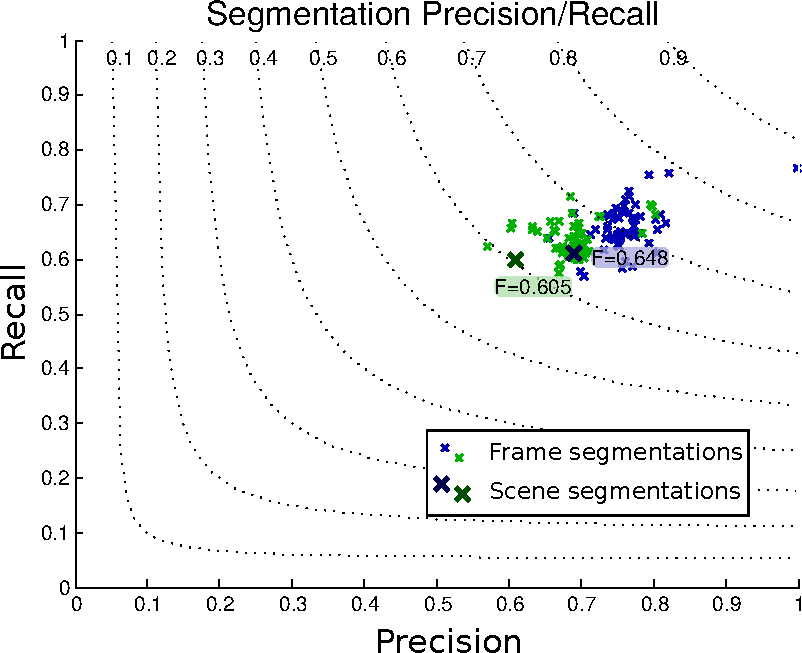
\includegraphics[width=0.4\textwidth]{figs/pipes2/frame_validation.pdf}
	      \\
	      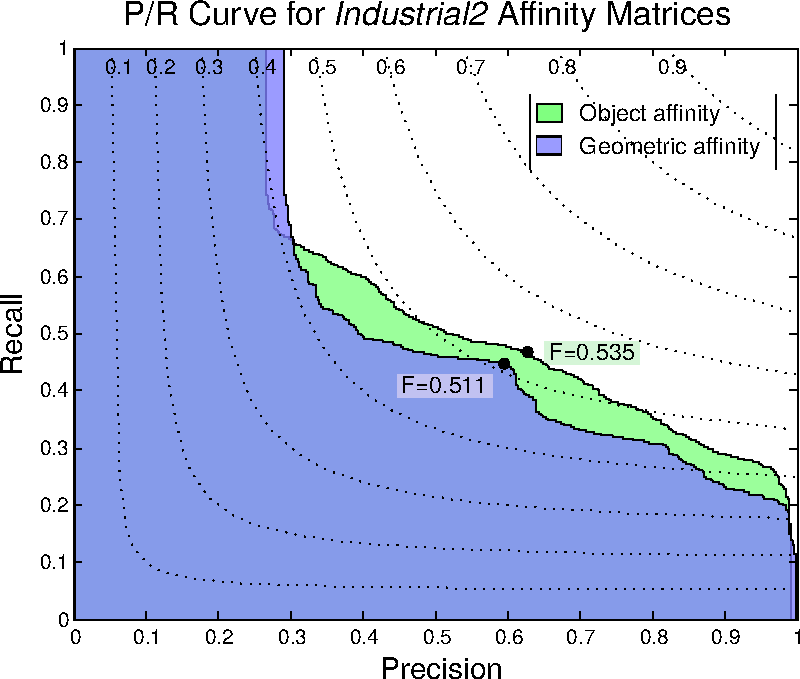
\includegraphics[width=0.4\textwidth]{figs/pipes3/validation.pdf}
	      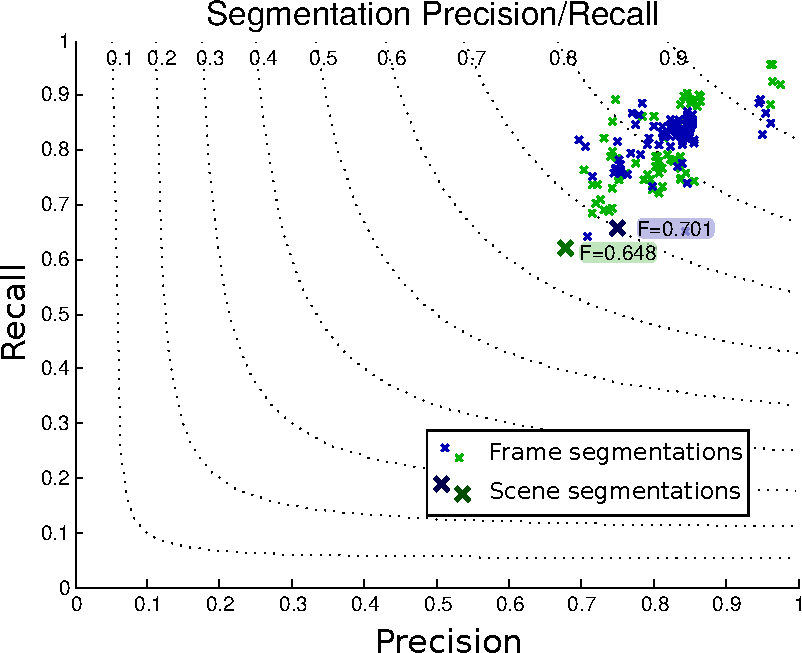
\includegraphics[width=0.4\textwidth]{figs/pipes3/frame_validation.pdf}
	      \end{tabular}
      }	
   }
\end{center}
{}
\caption{\small Quantitative evaluation of our segmentations vs. groundtruth.
The curves at left show 
precision and recall scores
induced by thresholding the affinity matrix at levels running from 0 to 1.
Highlighted points indicate the best threshold for clustering, vis-\`a-vis the ground truth.
At right, precision
and recall are computed from final segmentations, 
as well as from re-projected image segmentations.}
\label{fig:numericalEval}
{}
\end{figure}

\begin{figure}
\footnotesize
\centering
\begin{tabular}{c|c|c}
\quad Component & Time &\;Hardware\\
\hline
\begin{tabular}{l}
1. Dense Reconstruction \\
2. Image Segmentation \\
3. Construct Mesh \\
4. Compute Geodesics \\
5. Segmentation
\end{tabular} &
\begin{tabular}{c}
30Hz Realtime\\
3s / frame\\
.2s / frame\\
0.6s / traversal\\
1.2s
\end{tabular} &
\begin{tabular}{rcr}
&\rlap{GPU} \\
1&$\times$&CPU\\
1&$\times$&CPU\\
N&$\times$&CPU\\
1&$\times$&CPU
\end{tabular}
\end{tabular}

\caption{\small Approximate timings on the CoS sequence with a final mesh size of
roughly 57000
points. GPU is an Nvidia GTX 780. Note that traversing the mesh to compute geodesics for the sampled
subgraph is parallelized. Typically a subgraph of several hundred nodes is used.}
\label{fig:timing}
{}
\end{figure}

%-------------------------------------------------------------------------
%-------------------------------------------------------------------------
%-------------------------------------------------------------------------
\section{Conclusions}
\iffalse
\TODO{What is the justification for using the method of [2] for segmentation rather than segmenting the mesh directly?
}
\TODO{A discussion of why a mesh segmentation algorithm was not included as a baseline comparison
}
\TODO{An explanation of the role the Geman­McClure robust function plays}
\TODO{A discussion of what requirements were desired when developing the segmentation algorithm. It would be useful to state the specific role this algorithm could play in a practical application area.}
\TODO{How do you hand­select the scale for the geometric scale used as your baseline comparison (line 568)?}
\fi
We have presented a method to endow a scene, as densely reconstructed from monocular video, with a
metric that incorporates geometric and topological information as seen by the viewer, as well as
back-projected image statistics. While the latter are temporally inconsistent (they change with the
video), the way they change is spatially consistent, an observation key to defining distances or
affinities that allow us to partition the scene into coherent ``objects''. While one could employ
trained object detectors at the outset to arrive at a semantic segmentation of the scene (and, by
simple forward projection, of the video), we focus on low-level geometric and topological cues
first, to segment the image into coherent regions, where one could then deploy object detectors if
so desired. Semantic analysis of the scene involves object identities and relations, and knowledge
of scene geometry and topology is key to infer the latter. This is our focus in this work.
%Extensions include the integration with object labels, the incorporation of independent motions, and the inference of time-varying segmentations for
%dynamic scenes.
